% TODO checklist:
% - [x] Inspected ops/prometheus/alerts.yml (alerting rules configuration)
% - [x] Inspected ops/prometheus/recording_rules.yml (recording rules)
% - [x] Inspected ops/grafana/dashboards/health-overview.json (Grafana dashboard)
% - [x] Inspected ops/grafana/provisioning/datasources/datasource.yml
% - [x] Reviewed Q&A.md sections on observability and SLOs
% - [x] Reviewed README.md for observability overview

\section{Dashboards, SLOs, and Alerting}
\label{sec:dashboards-slos-alerting}

While the metrics subsystem provides the raw data foundation for observability, dashboards, Service Level Objectives (SLOs), and alerting rules transform this data into actionable operational intelligence. The Cineca Agentic Platform includes a pre-configured observability stack with Grafana dashboards and Prometheus alerting rules designed for enterprise deployment scenarios.

\subsection{Grafana Dashboard Architecture}

The platform ships with a ``Platform Health Overview'' dashboard that provides a unified view of system health across all components. The dashboard is provisioned automatically through Grafana's provisioning mechanism, ensuring consistent deployment across environments.

\subsubsection{Dashboard Layout and Panels}

The health overview dashboard is organized into four logical sections:

\begin{enumerate}
    \item \textbf{System Health Summary}: A single stat panel displaying overall system availability calculated as the average of all \texttt{up} metrics across monitored targets.
    
    \item \textbf{Component Status Timeline}: Time-series panels showing the health status evolution of critical components (PostgreSQL, Redis, Memgraph, providers, workers) and their latency trends over time.
    
    \item \textbf{Component Status Cards}: Individual stat panels for each component providing at-a-glance status with color-coded thresholds (green for OK, yellow for degraded, red/orange for error states).
    
    \item \textbf{Operational Metrics}: Detailed panels including provider health information tables and background job execution rates.
\end{enumerate}

\begin{figure}[ht]
\centering
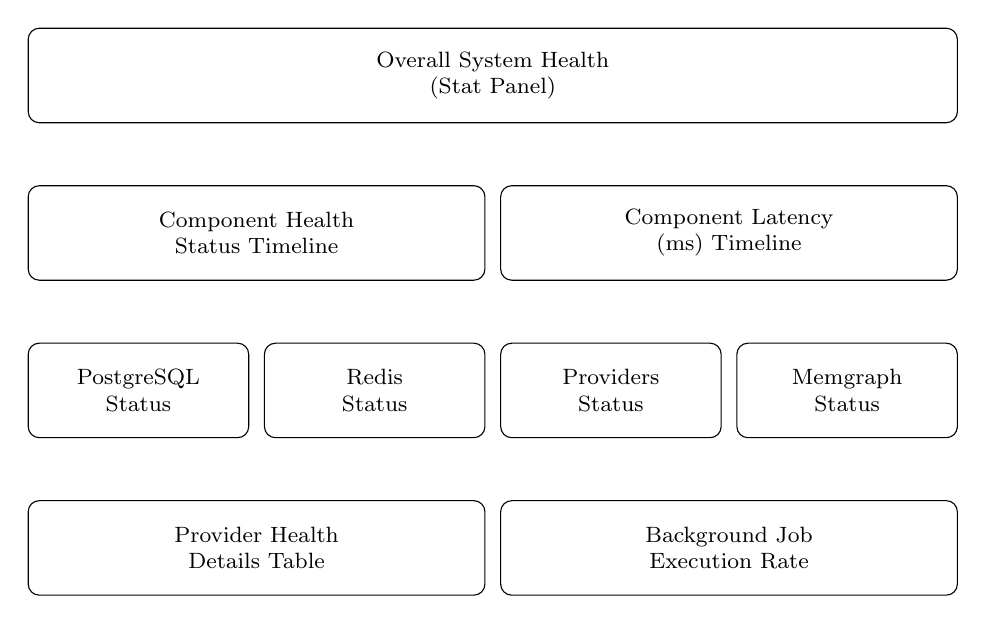
\begin{tikzpicture}[
    panel/.style={draw, rounded corners, minimum width=2.8cm, minimum height=1.2cm, font=\footnotesize, align=center},
    wide/.style={panel, minimum width=11.8cm},
    half/.style={panel, minimum width=5.8cm}
]
% Row 1 - Overall Health
\node[wide] at (0, 0) {Overall System Health\\(Stat Panel)};

% Row 2 - Timeseries
\node[half] at (-3, -2) {Component Health\\Status Timeline};
\node[half] at (3, -2) {Component Latency\\(ms) Timeline};

% Row 3 - Status Cards
\node[panel] at (-4.5, -4) {PostgreSQL\\Status};
\node[panel] at (-1.5, -4) {Redis\\Status};
\node[panel] at (1.5, -4) {Providers\\Status};
\node[panel] at (4.5, -4) {Memgraph\\Status};

% Row 4 - Details
\node[half] at (-3, -6) {Provider Health\\Details Table};
\node[half] at (3, -6) {Background Job\\Execution Rate};
\end{tikzpicture}
\caption{Platform Health Overview dashboard layout showing the logical organization of monitoring panels.}
\label{fig:dashboard-layout}
\end{figure}

\subsubsection{Component Status Visualization}

The dashboard uses a standardized three-state model for component health visualization:

\begin{itemize}
    \item \textbf{OK (0, Green)}: Component is healthy and operating within normal parameters.
    \item \textbf{Degraded (1, Yellow)}: Component is functional but experiencing issues that may affect performance or reliability.
    \item \textbf{Error (2, Red/Orange)}: Component is not functional or critically impaired; immediate attention required.
\end{itemize}

For informational components like Memgraph (which doesn't affect core readiness), the error state uses orange rather than red to indicate non-critical status.

\subsubsection{Latency Thresholds}

Component latency panels use graduated thresholds to provide visual cues about performance:

\begin{table}[ht]
\centering
\caption{Latency threshold configuration for component health visualization.}
\label{tab:latency-thresholds}
\begin{tabular}{lcccc}
\hline
\textbf{Threshold} & \textbf{Color} & \textbf{PostgreSQL} & \textbf{Redis} & \textbf{Providers} \\
\hline
Normal & Green & $<$ 100ms & $<$ 100ms & $<$ 100ms \\
Warning & Yellow & 100--500ms & 100--500ms & 100--500ms \\
Alert & Orange & 500--1000ms & 500--1000ms & 500--1000ms \\
Critical & Red & $>$ 1000ms & $>$ 1000ms & $>$ 1000ms \\
\hline
\end{tabular}
\end{table}

\subsection{Service Level Objectives (SLOs)}

The platform's alerting rules encode implicit SLOs that define acceptable service behavior. These SLOs are derived from the alert thresholds configured in \texttt{ops/prometheus/alerts.yml}:

\subsubsection{Availability SLOs}

\begin{table}[ht]
\centering
\caption{Availability-related Service Level Objectives.}
\label{tab:availability-slos}
\begin{tabular}{llp{6cm}}
\hline
\textbf{SLO} & \textbf{Target} & \textbf{Measurement} \\
\hline
Application Uptime & 99.9\% & \texttt{up\{job="app"\} == 1} over sliding window \\
Metrics Availability & 99.5\% & Presence of \texttt{process\_start\_time\_seconds} metric \\
Target Reachability & 99.9\% & All Prometheus targets reporting \texttt{up == 1} \\
\hline
\end{tabular}
\end{table}

\subsubsection{Performance SLOs}

\begin{table}[ht]
\centering
\caption{Performance-related Service Level Objectives.}
\label{tab:performance-slos}
\begin{tabular}{llp{6cm}}
\hline
\textbf{SLO} & \textbf{Target} & \textbf{Measurement} \\
\hline
HTTP P95 Latency & $<$ 750ms & 95th percentile of \texttt{http\_request\_duration\_seconds} \\
Error Rate & $<$ 5\% & Ratio of 5xx responses to total requests \\
Job Creation P95 & $<$ 2s & 95th percentile of \texttt{job\_create\_duration\_seconds} \\
Job Retrieval P95 & $<$ 500ms & 95th percentile of \texttt{job\_get\_duration\_seconds} \\
\hline
\end{tabular}
\end{table}

\subsubsection{Resource SLOs}

\begin{table}[ht]
\centering
\caption{Resource utilization Service Level Objectives.}
\label{tab:resource-slos}
\begin{tabular}{llp{6cm}}
\hline
\textbf{SLO} & \textbf{Target} & \textbf{Measurement} \\
\hline
Memory Usage & $<$ 500 MiB & \texttt{process\_resident\_memory\_bytes} \\
CPU Utilization & $<$ 90\% core & \texttt{rate(process\_cpu\_seconds\_total[5m])} \\
SSE Connections & $<$ 100 & \texttt{sse\_connections\_active} gauge \\
\hline
\end{tabular}
\end{table}

\subsection{Alerting Rules}

The platform includes a comprehensive set of Prometheus alerting rules organized into five rule groups:

\subsubsection{Availability and Liveness Alerts}

These alerts detect service unavailability and infrastructure issues:

\begin{lstlisting}[language=yaml, caption={Critical availability alerts}]
- alert: AppInstanceDown
  expr: up{job="app"} == 0
  for: 2m
  labels:
    severity: critical
    team: platform
  annotations:
    summary: "App instance is down"
    runbook: "Check docker compose status and app logs"

- alert: AppMetricsMissing
  expr: absent(process_start_time_seconds{job="app"})
  for: 10m
  labels:
    severity: warning
  annotations:
    summary: "No app metrics found"
    description: "Metrics endpoint may be misconfigured"
\end{lstlisting}

\subsubsection{HTTP Health and Error Alerts}

These alerts monitor API health and user-facing error rates:

\begin{lstlisting}[language=yaml, caption={HTTP error rate alerting rule}]
- alert: AppHigh5xxErrorRate
  expr: |
    sum(rate(http_requests_total{job="app",status=~"5.."}[5m]))
    /
    clamp_min(sum(rate(http_requests_total{job="app"}[5m])), 1e-9)
    > 0.05
  for: 10m
  labels:
    severity: critical
  annotations:
    summary: "High 5xx error rate (>5%)"
    runbook: "Check app logs and recent deploys"

- alert: AppHighLatencyP95
  expr: |
    histogram_quantile(0.95,
      sum by (le) (rate(http_request_duration_seconds_bucket{job="app"}[5m]))
    ) > 0.75
  for: 10m
  labels:
    severity: warning
  annotations:
    summary: "High latency (P95 > 750ms)"
\end{lstlisting}

\subsubsection{Resource Usage Alerts}

These alerts track process resource consumption:

\begin{lstlisting}[language=yaml, caption={Resource monitoring alerts}]
- alert: AppHighMemoryUsage
  expr: process_resident_memory_bytes{job="app"} > 500 * 1024 * 1024
  for: 10m
  labels:
    severity: warning
  annotations:
    summary: "High memory usage (>500MiB)"
    runbook: "Inspect memory profiles and caches"

- alert: AppHighCPUUsage
  expr: rate(process_cpu_seconds_total{job="app"}[5m]) > 0.9
  for: 10m
  labels:
    severity: warning
  annotations:
    summary: "High CPU usage (>90% of a core)"
\end{lstlisting}

\subsubsection{Job Store Health Alerts}

These alerts monitor the Redis-based job storage system:

\begin{lstlisting}[language=yaml, caption={Job store alerting rules}]
- alert: JobStoreHighCreateLatency
  expr: |
    histogram_quantile(0.95,
      sum by (backend, le) (rate(job_create_duration_seconds_bucket[5m]))
    ) > 2.0
  for: 10m
  labels:
    severity: warning
  annotations:
    summary: "High job creation latency (P95 > 2s)"

- alert: RedisConnectionErrors
  expr: rate(redis_connection_errors_total[5m]) > 0.1
  for: 5m
  labels:
    severity: critical
  annotations:
    summary: "Redis connection errors detected"
    runbook: "Check Redis health with redis-cli PING"
\end{lstlisting}

\subsubsection{SSE and Streaming Alerts}

These alerts monitor the Server-Sent Events streaming infrastructure:

\begin{lstlisting}[language=yaml, caption={SSE streaming alerts}]
- alert: SSETooManyGaps
  expr: rate(sse_gap_events_total[10m]) > 1
  for: 15m
  labels:
    severity: warning
  annotations:
    summary: "High SSE gap rate (ring buffer eviction)"
    runbook: "Consider increasing SSE_RING_SIZE"

- alert: SSEHighConnectionCount
  expr: sse_connections_active > 100
  for: 10m
  labels:
    severity: info
  annotations:
    summary: "High active SSE connection count (>100)"
\end{lstlisting}

\subsection{Alert Severity Classification}

The platform uses a four-level severity classification aligned with industry practices:

\begin{table}[ht]
\centering
\caption{Alert severity levels and expected response.}
\label{tab:alert-severity}
\begin{tabular}{llp{8cm}}
\hline
\textbf{Severity} & \textbf{Response Time} & \textbf{Description} \\
\hline
\texttt{critical} & Immediate & Service-affecting issues requiring immediate intervention \\
\texttt{warning} & Hours & Issues that may escalate if unaddressed \\
\texttt{info} & Days & Informational alerts for capacity planning \\
\texttt{notice} & Weekly & Trends and patterns for review \\
\hline
\end{tabular}
\end{table}

\subsection{Recommended Dashboard Extensions}

Organizations deploying the platform are encouraged to extend the base dashboard with additional panels tailored to their operational needs:

\begin{itemize}
    \item \textbf{Tenant-Specific Views}: Panels filtered by \texttt{tenant\_id} label for multi-tenant cost attribution and SLA tracking.
    
    \item \textbf{LLM Provider Comparison}: Side-by-side latency and error rate comparisons across providers to inform failover decisions.
    
    \item \textbf{Cost Attribution}: Panels computing estimated costs using token counters and configured pricing.
    
    \item \textbf{Intent Classification Analysis}: Breakdown of classification sources (pattern, catalog, LLM) and confidence distributions.
    
    \item \textbf{Graph Query Performance}: NL-to-Cypher pipeline metrics including generation latency and validation pass rates.
\end{itemize}

\subsection{Alertmanager Integration}

The platform's Prometheus configuration includes a placeholder for Alertmanager integration:

\begin{lstlisting}[language=yaml, caption={Alertmanager configuration placeholder}]
# alerting:
#   alertmanagers:
#     - static_configs:
#         - targets: ["alertmanager:9093"]
\end{lstlisting}

Production deployments should configure Alertmanager to route alerts to appropriate notification channels (email, Slack, PagerDuty, OpsGenie) based on severity and team ownership labels.

